\section{Invisibly} \label{invisibly}
Invisibly ist eine Plattform, bei der Benutzer ihre persönlichen Daten zur lizenzierten Freigabe bereitstellen können. Sie befindet sich derzeit noch in der Beta-Phase und ist bisher ausschließlich in Amerika verfügbar.

\subsection{Ziel}
Die Plattform hatte ursprünglich das Ziel, bezahlungspflichtige Artikel leichter zugänglich zu machen. Benutzer der Webseite sollten Werbung ansehen und dafür Token erhalten, welche sie anschließend für den Zugang zu einzelnen Publikationen von Nachrichtenseiten und Wissenschaftsmagazinen ausgeben konnten -- ohne bei den einzelnen Diensten beispielsweise ein Abonnement abzuschließen. Da diese Idee nur wenige Personen überzeugte, wurde das Konzept überarbeitet. \cite{techRadarInvisibly_2021} \newline

\noindent Heute verfolgt Invisibly das Ziel, seine Benutzer mit einem fairen Anteil am Wert zu beteiligen, der bei der Verarbeitung persönlicher Daten entsteht. Die Plattform versucht dies aktuell auf zwei verschiedene Wege. Im Gegensatz zu anderen Plattformen, die Inhalte strategisch platzieren, versucht Invisibly als erstes seinen Benutzern auf Basis der freiwillig geteilten Daten hochwertige Inhalte zu präsentieren, die sie tatsächlich sehen wollen: \begin{quote}
    \textit{``We are creating an AI-powered platform with a feed that`s a true extension of you, rather than a feed strategically curated and targeted at you by the Big Tech and brands.'' \cite{invisiblyWhyPay_2021}}
\end{quote} Im zweiten Schritt zielt Invisibly darauf ab, seine Benutzer direkt am Verkauf der persönlichen Daten zu beteiligen, indem sie ihnen regelmäßig Geld auszahlt. \cite{invisiblyWhyPay_2021} Der Gründer von Invisibly, Jim McKelvey, beschreibt seine Plattform in einem Interview wie folgt: \begin{quote}
    \textit{``We basically act as your agent. We try to sell you to advertisers and we give you the money. We ask how much you are willing to sell, package it up and sell it to the highest bidder.'' \cite{techRadarInvisibly_2021}}
\end{quote} Die Plattform verkauft die Rohdaten ihrer Nutzer jedoch nicht direkt -- stattdessen lizenziert Invisibly die Daten ihrer Nutzer. Auf diese Weise bleibt die individuelle Person Eigentümer der Daten und kann selbst bestimmen, welche Daten sie freigeben möchte. \cite{invisiblyGetPaid_2021} Anschließend vermittelt Invisibly die Lizenzen an Werbetreibende für Dienste und Produkte, die am besten zum jeweiligen Benutzer passen. Sie erhalten mit einer Lizenz solange Zugriff auf die persönlichen Daten, bis ein Benutzer seine Lizenz widerruft und somit die Freigabe beendet. Der Zugriff auf eine Datenquelle wird widerrufen, indem Benutzer die Datenquelle aus ihrem Invisibly-Profil unter \textit{Data Vault} entfernen. Um die Daten vollständig von der Invisibly-Plattform zu löschen, muss der Betreiber jedoch direkt konaktiert werden (siehe Abbildung \ref{fig:invisiblyProfile}). \newline

\noindent Der Vorteil für Unternehmen besteht darin, dass Invisibly sie durch den Kauf von Lizenzen mit den Individuen zusammenbringt, die potentiell am besten zu deren Produkten passen. \cite{techRadarInvisibly_2021} Dabei ist es wichtig zu erwähnen, dass Benutzer von Invisibly ihre Daten freiwillig zur Lizenzierung freigeben und deshalb wahrscheinlich von einer Vermittlung an Dritte nicht abgeneigt sind. \newline

\noindent Im Folgenden wird erklärt, wie Individuen ihre persönlichen Daten bei Invisibly zu Geld machen können.

\subsection{Daten auf der Invisibly-Plattform monetarisieren}
Benutzer sammeln bei Invisibly Punkte, wenn sie persönliche Daten mit der Plattform teilen. Gesammelte Punkte können später in US-Dollar umgerechnet und ausgezahlt werden. Derzeit gibt es drei verschiedene Möglichkeiten, Punkte zu sammeln: \newline

\noindent \textbf{Datenquellen verlinken:} Die meisten Punkte sammeln Benutzer, indem sie verschiedene Datenquellen in ihrem Invisibly-Profil hinterlegen. Für jede Datenquelle wird monatlich ein fester Betrag an Punkten gutgeschrieben, ähnlich wie bei einem passiven Einkommen. \cite{pymntsInvisibly_2021} Das Verknüpfen eines Bankkontos wird beispielsweise mit \textit{75 Punkten} pro Monat vergütet, wobei Werbepartner so Zugriff auf sämtliche Transaktionsdaten erhalten. Andererseits lassen sich verschiedene soziale Netzwerke bei Invisibly hinterlegen. Für jeden Account erhält ein Benutzer monatlich \textit{25 Punkte} und es werden aktuell die Plattformen Instagram, Twitter, TikTok, LinkedIn und Pinterest unterstützt. Zum Schluss bietet Invisibly eine Browser-Erweiterung an, welche den Verlauf der besuchten Webseiten aufzeichnet. Mit ihr sammeln Benutzer \textit{200 Punkte} pro Monat. \cite{instagramInvisibly_2021, lifewireInvisibly_2021} Abbildung \ref{fig:invisiblyProfile} zeigt im zweiten Screenshot den Tab \textit{Data Vault} der Invisibly-App, in welchem die hinterlegten Datenquellen verwaltet werden können. \newline

\begin{figure}[!ht]
	\centering
	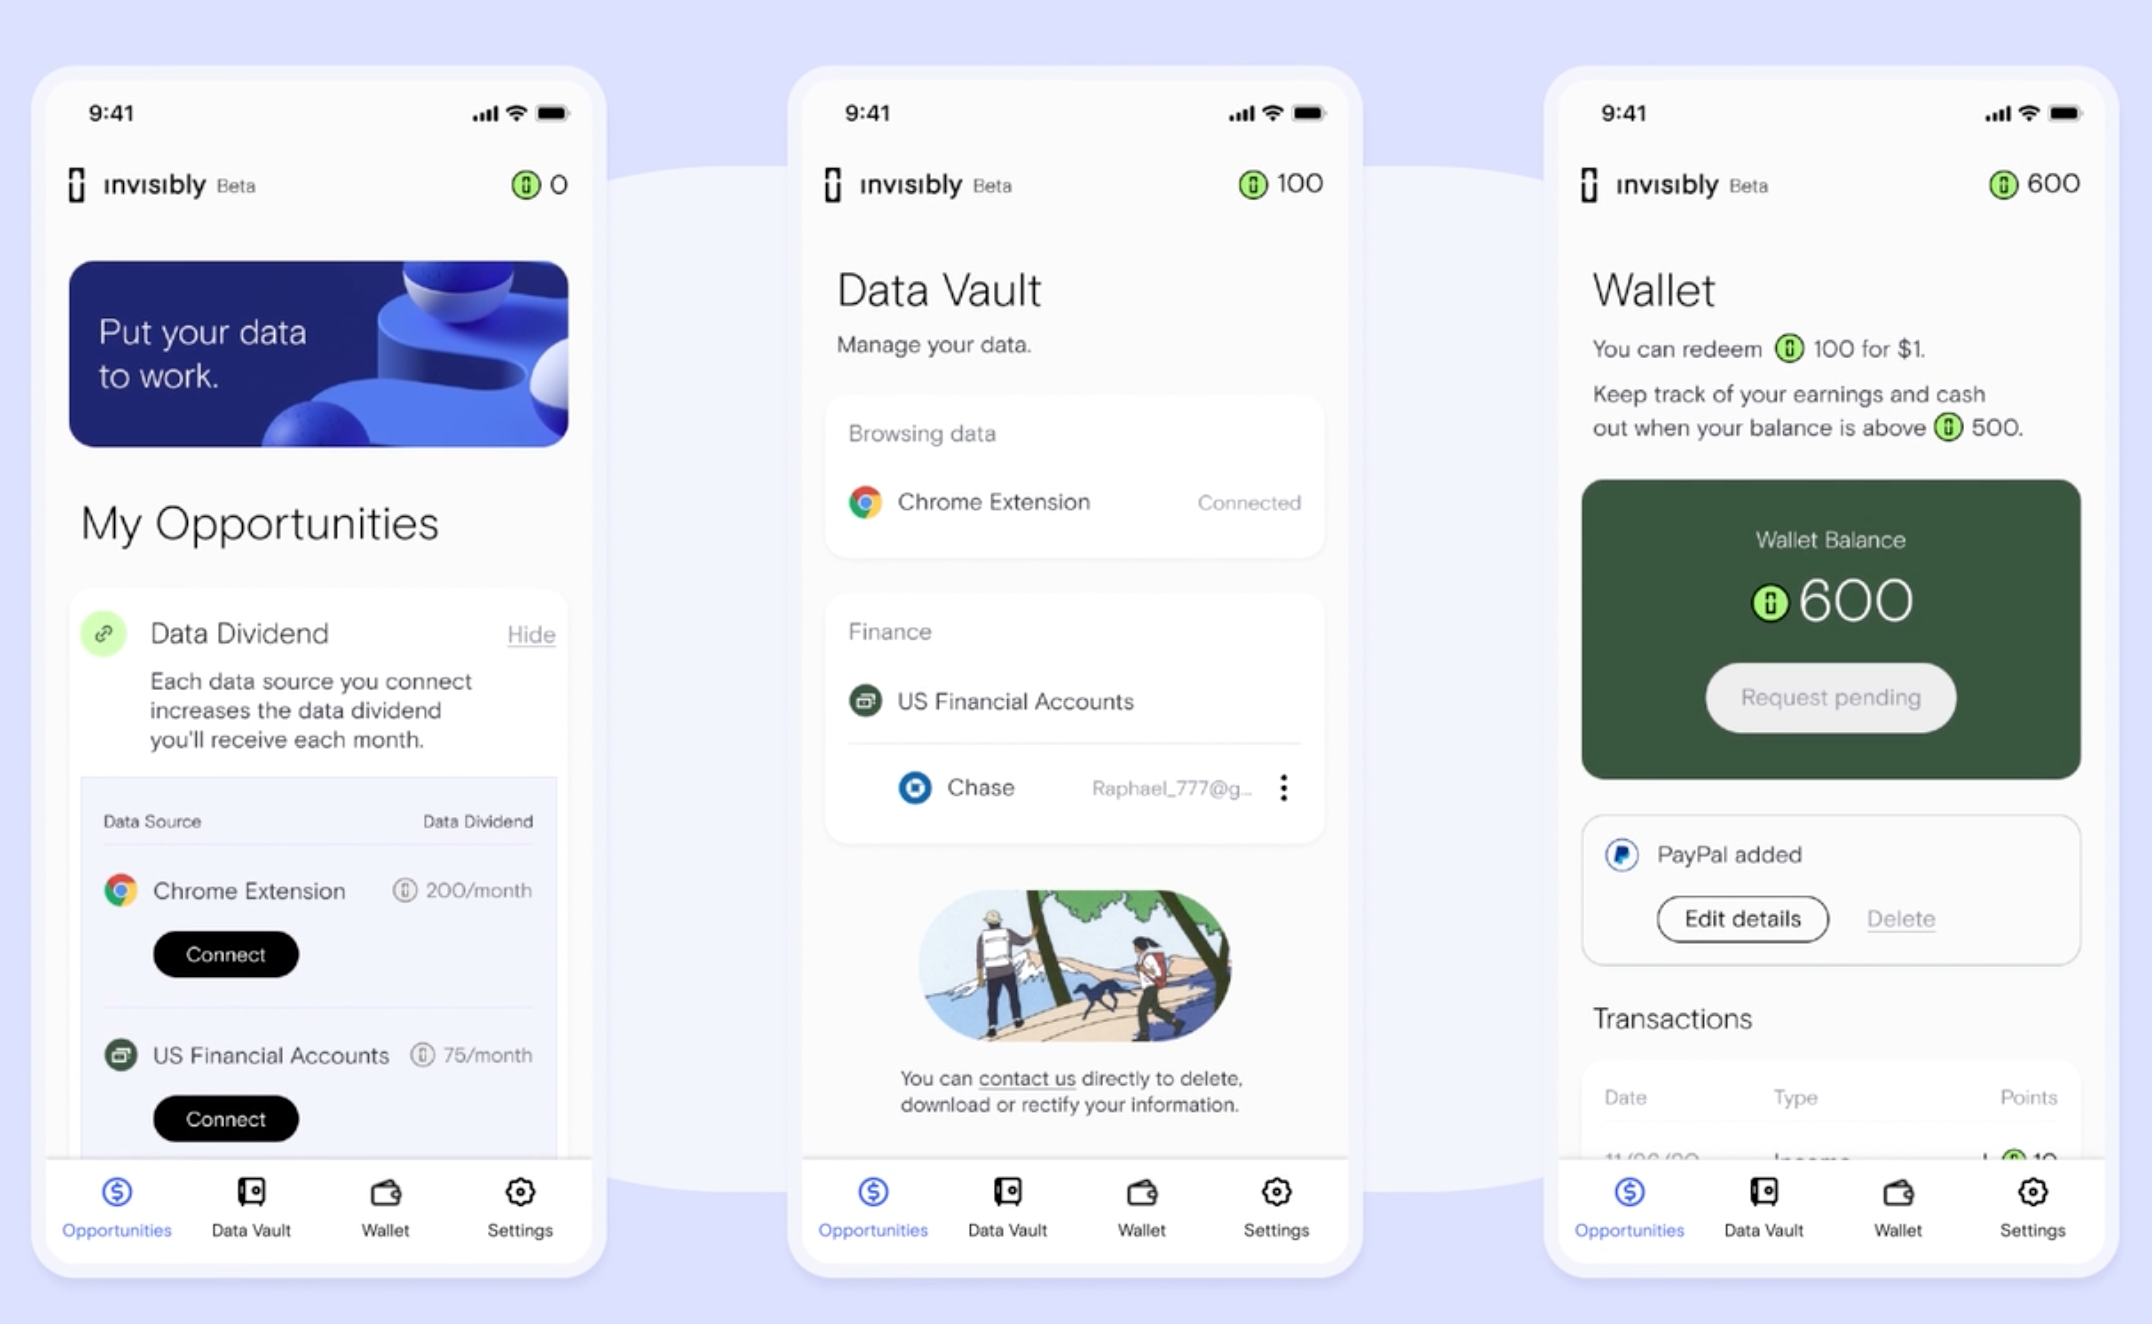
\includegraphics[width=\textwidth]{invisibly_profile}
	\caption{Ansichten in der mobilen Invisibly-App: My Opportunities, Data Vault und Wallet \cite{behanceInvisibly_2021}}
	\label{fig:invisiblyProfile}
\end{figure}
\FloatBarrier

\noindent \textbf{Fragen zur Person:} Benutzer können ihr Invisibly-Profil vervollständigen, indem sie verschiedene Fragen zu ihrer Person beantworten. So fragt die Webseite beispielsweise nach dem Geschlecht, dem höchsten Bildungsabschluss oder ob man Kinder hat. Jede Antwort wird dabei mit \textit{einem Punkt} vergütet. \cite{instagramInvisibly_2021} \newline

\noindent \textbf{Persönliches Feed:} Das persönliche Feed ist Invisibly's Vision von einer besseren Alternative zu Facebook und ähnlichen Beispielen. Das Feed enthält relevante Beiträge, die auf Basis der freiwillig geteilten, persönlichen Daten von verschiedenen Datenquellen ausgewählt und angezeigt werden. Diese Beiträge bestehen aus Bildern mit kurzen Texten und verweisen auf Dienstleistungen und Produkte von Werbetreibenden, wie beispielsweise kaufbare Gebrauchsgegenstände, Reise- und Ausflugsziele, Veranstaltungen, Gutscheine oder sonstige Angebote in Online-Shops und vieles mehr. Jeder Beitrag kann mit einem \textit{Like} oder \textit{Dislike} markiert werden -- auf diese Weise sammelt Invisibly Daten über persönliche Interessen und kann Vorschläge noch besser auf jede Person zuschneiden. Benutzer erhalten im Gegenzug für jeden Like oder Dislike \textit{einen Punkt}, wobei die maximale Anzahl an Punkten hier auf 20 Punkte pro Tag begrenzt ist. \cite{invisiblyWhyPay_2021} \newline

\noindent Das in Abbildung \ref{fig:invisiblyProfile} gezeigte erste Screenshot der Invisibly-App zeigt die Ansicht \textit{My Opportunities}, in welcher dem Benutzer noch nicht erledigte Möglichkeiten zum Sammeln von Punkten vorgeschlagen werden. An erster Stelle werden die Datenquellen aufgelistet, für welche noch kein Account hinterlegt ist, gefolgt von Fragen zur Person und dem persönlichen Feed. \newline

\noindent Die gesammelten Punkte können abschließend direkt in Geld umgewandelt werden: 100 Punkte entsprechen \$1 und eine Auszahlung ist ab 500 Punkten möglich. \cite{invisiblyWhyPay_2021} Eine Auszahlung ist über das \textit{Wallet} möglich, welche sowohl in der mobilen Version als auch über die in Abbildung \ref{fig:invisiblyWallet} dargestellte Webseite aufrufbar ist. Hier können Benutzer neben ihrem aktuellen Punktestand auch einen Verlauf der gutgeschriebenen Punkte einsehen. Eine Auszahlung ist derzeit ausschließlich über den amerikanischen Zahlungsdienstleister PayPal möglich. \newline

\begin{figure}[!ht]
	\centering
	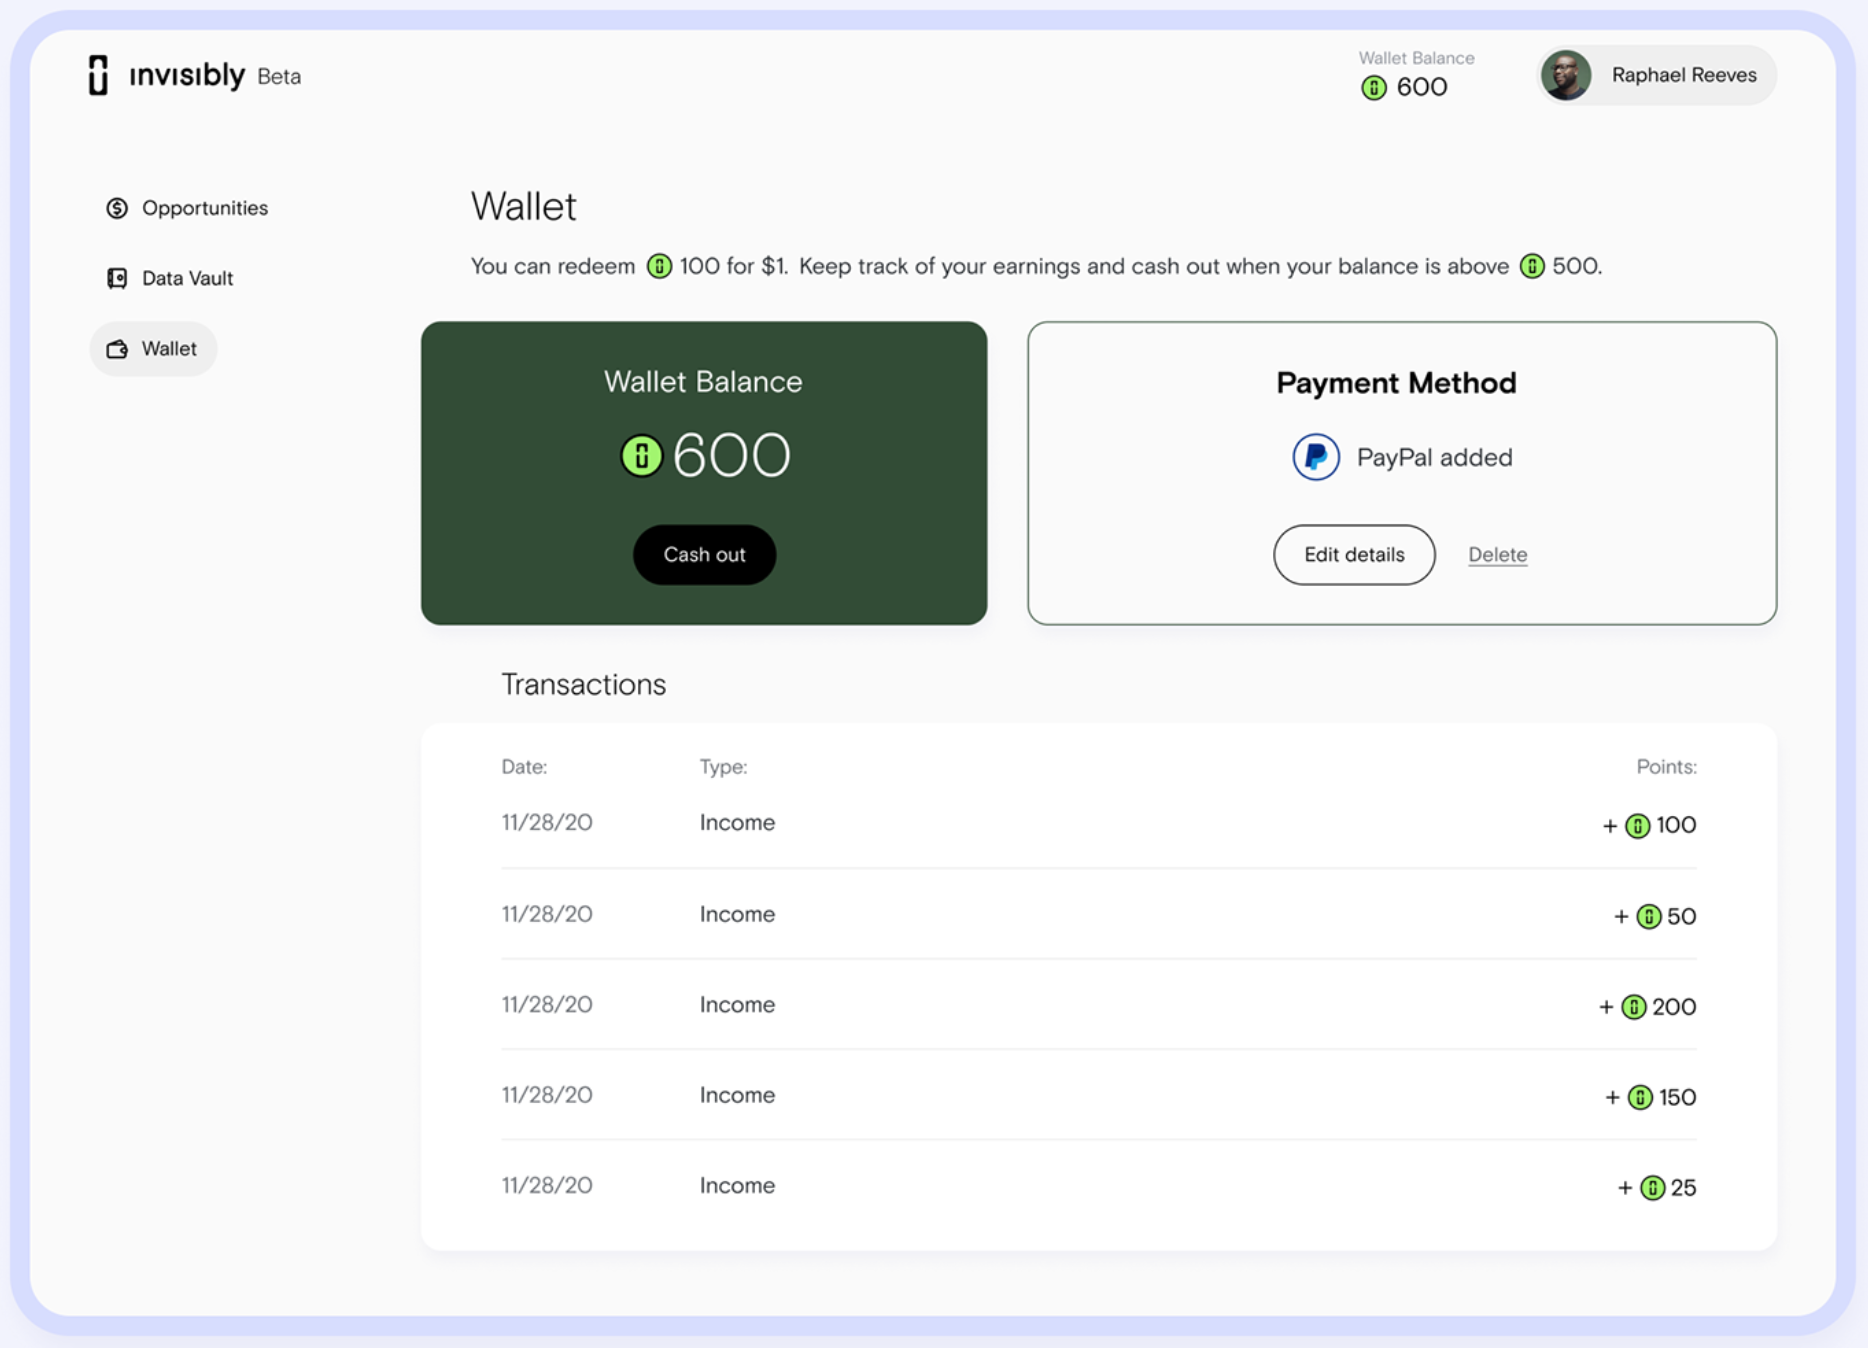
\includegraphics[width=0.9\textwidth]{invisibly_wallet}
	\caption{Wallet mit Kontostand und Verlauf der gesammelten Punkte \cite{behanceInvisibly_2021}}
	\label{fig:invisiblyWallet}
\end{figure}
\FloatBarrier

\noindent Die Monetarisierung von persönlichen Daten bringt Invisibly's Nutzern derzeit ca. \$60 bis \$100 im Jahr, abhängig von der Anzahl verlinkter Datenquellen. Das liegt daran, dass aktuell ein flaches Bezahlmodell verwendet wird, bei dem jeder Nutzer gleich viel Geld bzw. Punkte für seine persönlichen Daten bekommt -- unabhängig davon, wieviel die Daten konkret für Werbetreibende wert sind. In Zukunft soll ein kompetitives Modell zum Einsatz kommen, bei dem Personen eine höhere Dividende erhalten, wenn die Daten für Werbetreibende mehr wert sind. \cite{pymntsInvisibly_2021} Der Gründer von Invisibly geht davon aus, dass ein schnell wachsender Marktplatz mit mehr Werbetreibenden und Individuen in wenigen Jahren bereits \$1000 pro Jahr für Nutzer des Dienstes erwirtschaften kann. \cite{techRadarInvisibly_2021} 
